\input{../utils/preamble}
\createdgmtitle{11}
%--------------------------------------------------------------------------------
\begin{document}
%--------------------------------------------------------------------------------
\begin{frame}
%\thispagestyle{empty}
\titlepage
\end{frame}
%=======
\begin{frame}{Recap of previous lecture}
	\begin{block}{Kantorovich-Rubinstein duality}
		\vspace{-0.2cm}
		\[
			W(\pi || p) = \frac{1}{K} \max_{\| f \|_L \leq K} \left[ \bbE_{\pi(\bx)} f(\bx)  - \bbE_{p(\bx)} f(\bx)\right],
		\]
		where $\| f \|_L \leq K$ are $K-$Lipschitz continuous functions ($f: \cX \rightarrow \bbR$).
	\end{block}
	\begin{block}{Gradient penalty}
		\vspace{-0.3cm}
		\[
			W(\pi || p) = \underbrace{\bbE_{\pi(\bx)} f(\bx)  - \bbE_{p(\bx)} f(\bx)}_{\text{original critic loss}} + \lambda \underbrace{\bbE_{U[0, 1]} \left[ \left( \| \nabla_{\hat{\bx}} f(\hat{\bx}) \|_2 - 1 \right) ^ 2\right]}_{\text{gradient penalty}}.
		\]
		Samples $\hat{\bx}_t = t \bx + (1 - t) \by$ with $t \in [0, 1]$ are uniformly sampled along straight lines between pairs of points: $\bx$ from the data distribution $\pi(\bx)$ and $\by$ from the generator distribution $p(\bx | \btheta)$.
	\end{block}
	\myfootnote{
	\href{https://arxiv.org/abs/1701.07875}{Arjovsky M., Chintala S., Bottou L. Wasserstein GAN, 2017} \\
	\href{https://arxiv.org/abs/1704.00028}{Gulrajani I. et al. Improved Training of Wasserstein GANs, 2017} }
\end{frame}
%=======
\begin{frame}{Recap of previous lecture}
	\vspace{-0.3cm}
	\[
		f(\bx, \bphi) = \bW_{K+1} a_K (\bW_K a_{K-1}(\dots a_1(\bW_1 \bx) \dots)).
	\]
	\vspace{-0.3cm}
	\begin{itemize}
		\item $a_k$ is a pointwise nonlinearities. We assume that $\| a_k \|_L = 1$ (it holds for ReLU).
		\item $\mathbf{g}(\bx) = \bW \bx$ is a linear transformation ($\nabla \mathbf{g}(\bx) = \bW$).
		\[
			\| \mathbf{g} \|_L = \sup_\bx \sigma( \nabla \mathbf{g}(\bx)) = \sigma(\bW).
		\]
	\end{itemize}
	\vspace{-0.3cm}
	\begin{block}{Critic spectral norm}
		\vspace{-0.3cm}
		\[
			\| f \|_L \leq \| \bW_{K+1}\| \cdot \prod_{k=1}^K  \| a_k \|_L \cdot \| \bW_k \| = \prod_{k=1}^{K+1} \sigma(\bW_k).
		\]
		\vspace{-0.2cm}
	\end{block}
	\begin{block}{Spectral Normalization GAN}
	If we replace the weights in the critic $f(\bx, \bphi)$ by $\bW^{SN}_k = \bW_k / \sigma(\bW_k)$, we will get $\| f\|_L \leq 1.$ \\
	\end{block}
	 Power iteration approximates the value of $\sigma(\bW)$.
	
	\myfootnotewithlink{https://arxiv.org/abs/1802.05957}{Miyato T. et al. Spectral Normalization for Generative Adversarial Networks, 2018}

\end{frame}
%=======
\begin{frame}{Recap of previous lecture}
	\begin{block}{What is a divergence?}
		Let $\cS$ be the set of all possible probability distributions. Then $D: \cS \times \cS \rightarrow \bbR$ is a divergence if 
		\begin{itemize}
			\item $D(\pi || p) \geq 0$ for all $\pi, p \in \cS$;
			\item $D(\pi || p) = 0$ if and only if $\pi \equiv p$.
		\end{itemize}
	\end{block}
	\vspace{-0.2cm}
	\begin{block}{f-divergence minimization}
		\vspace{-0.3cm}
		\[
		D_f(\pi || p) = \bbE_{p(\bx)}  f\left( \frac{\pi(\bx)}{p(\bx)} \right) \rightarrow \min_p.
		\]
	\end{block}
	\vspace{-0.3cm}
	\begin{block}{Variational divergence estimation}
		\vspace{-0.3cm}
		\[
			D_f(\pi || p) \geq \sup_{T \in \cT} \left[\bbE_{\pi}T(\bx) -  \bbE_p f^*(T(\bx)) \right],
		\]
		\vspace{-0.4cm}
		where $ f^*(t) = \sup_{u \in \text{dom}_f} \left( ut - f(u) \right)$ -- Fenchel conjugate.
	\end{block}
	\myfootnotewithlink{https://arxiv.org/abs/1606.00709}{Nowozin S., Cseke B., Tomioka R. f-GAN: Training Generative Neural Samplers using Variational Divergence Minimization, 2016}
\end{frame}
%=======
\begin{frame}{Recap of previous lecture}
	Let take some pretrained image classification model to get the conditional label distribution $p(y | \bx)$ (e.g. ImageNet classifier).
	\begin{block}{Evaluation of likelihood-free models}
		\begin{itemize}
			\item Sharpness $\Rightarrow$ low $H(y | \bx) = - \sum_{y} \int_{\bx} p(y, \bx) \log p(y | \bx) d\bx$.
			\item Diversity $\Rightarrow$ high $H(y)  = - \sum_{y} p(y) \log p(y)$.
		\end{itemize}
	\end{block}
	\vspace{-0.3cm}
	\begin{block}{Inception Score}
		\vspace{-0.2cm}
		\[
			IS = \exp(H(y) - H(y | \bx)) = \exp \left( \bbE_{\bx} KL(p(y | \bx) || p(y)) \right)
		\]
		\vspace{-0.5cm}
	\end{block}
	\begin{block}{Frechet Inception Distance}
		\vspace{-0.3cm}
		\[
			D^2 (\pi, p) = \| \mathbf{m}_{\pi} - \mathbf{m}_{p}\|_2^2 + \text{Tr} \left( \bC_{\pi} + \bC_p - 2 \sqrt{\bC_{\pi} \bC_p} \right).
		\]
		\vspace{-0.5cm}
	\end{block}
	FID is related to moment matching.
	
	\myfootnote{\href{https://arxiv.org/abs/1606.03498}{Salimans T. et al. Improved Techniques for Training GANs, 2016} \\
	\href{https://arxiv.org/abs/1706.08500}{Heusel M. et al. GANs Trained by a Two Time-Scale Update Rule Converge to a Local Nash Equilibrium, 2017} }
\end{frame}
%=======
\begin{frame}{Precision-Recall}
	\begin{block}{What do we want from samples}
		\begin{itemize}
			\item \textbf{Sharpness}: generated samples should be of high quality.
			\item \textbf{Diversity}: their variation should match that observed in the training set.
		\end{itemize}
	\end{block}
	\vspace{-0.5cm}
	\begin{figure}
		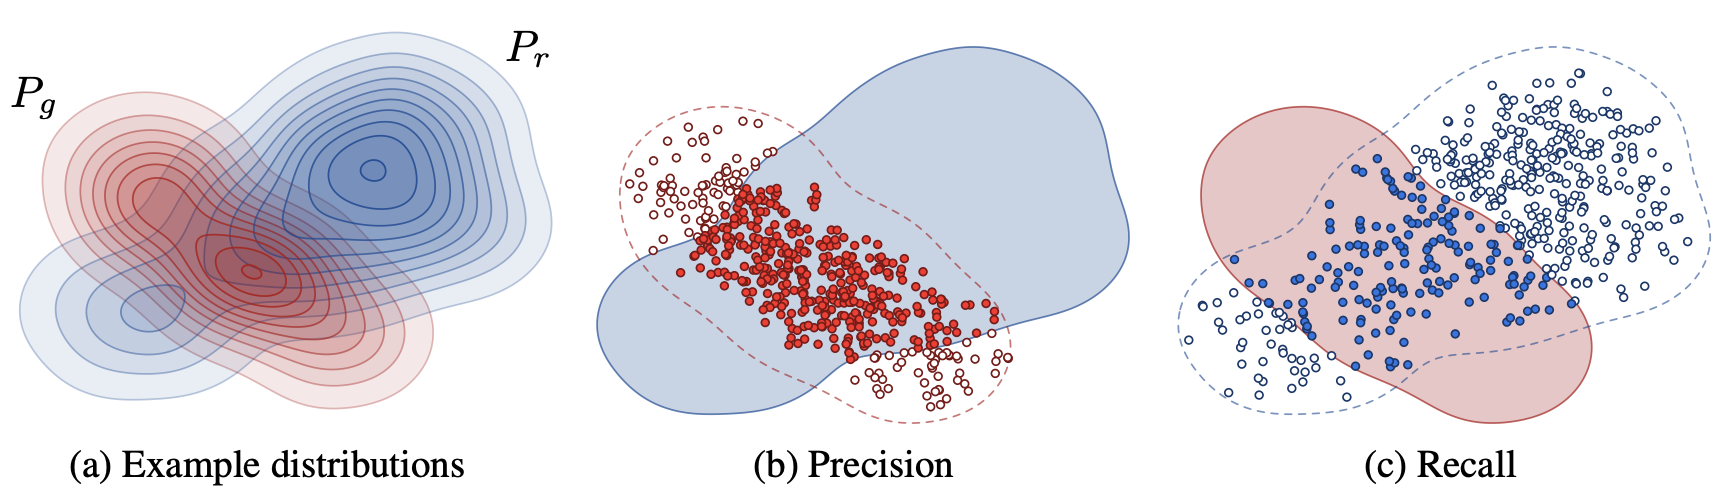
\includegraphics[width=0.95\linewidth]{figs/pr_curve}
	\end{figure}
	\vspace{-0.3cm}
	\begin{itemize}
		\item \textbf{Precision} denotes the fraction of generated images that are realistic.
		\item \textbf{Recall} measures the fraction of the training data manifold covered by the generator.
	\end{itemize}
	\myfootnotewithlink{https://arxiv.org/abs/1904.06991}{Kynkäänniemi T. et al. Improved precision and recall metric for assessing generative models, 2019}
\end{frame}
%=======
\begin{frame}{Precision-Recall}
	\begin{figure}
		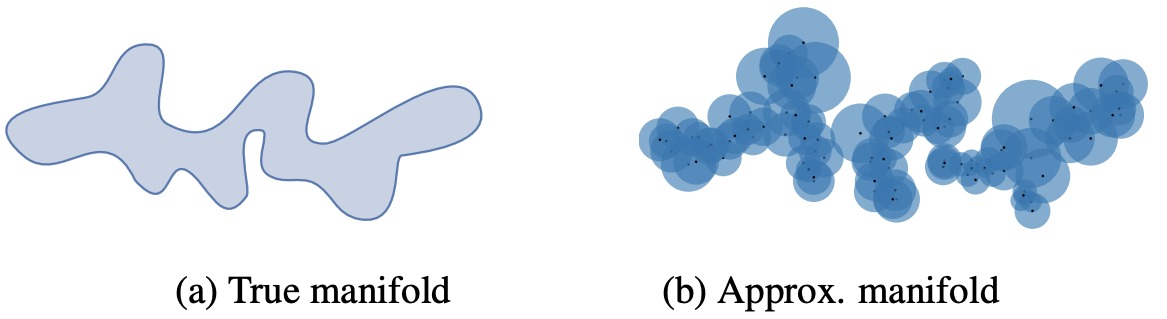
\includegraphics[width=0.7\linewidth]{figs/pr_k_nearest}
	\end{figure}
	\myfootnotewithlink{https://arxiv.org/abs/1904.06991}{Kynkäänniemi T. et al. Improved precision and recall metric for assessing generative models, 2019}
\end{frame}
%=======
\begin{frame}{Evolution of GANs}
	\begin{figure}
		\centering
		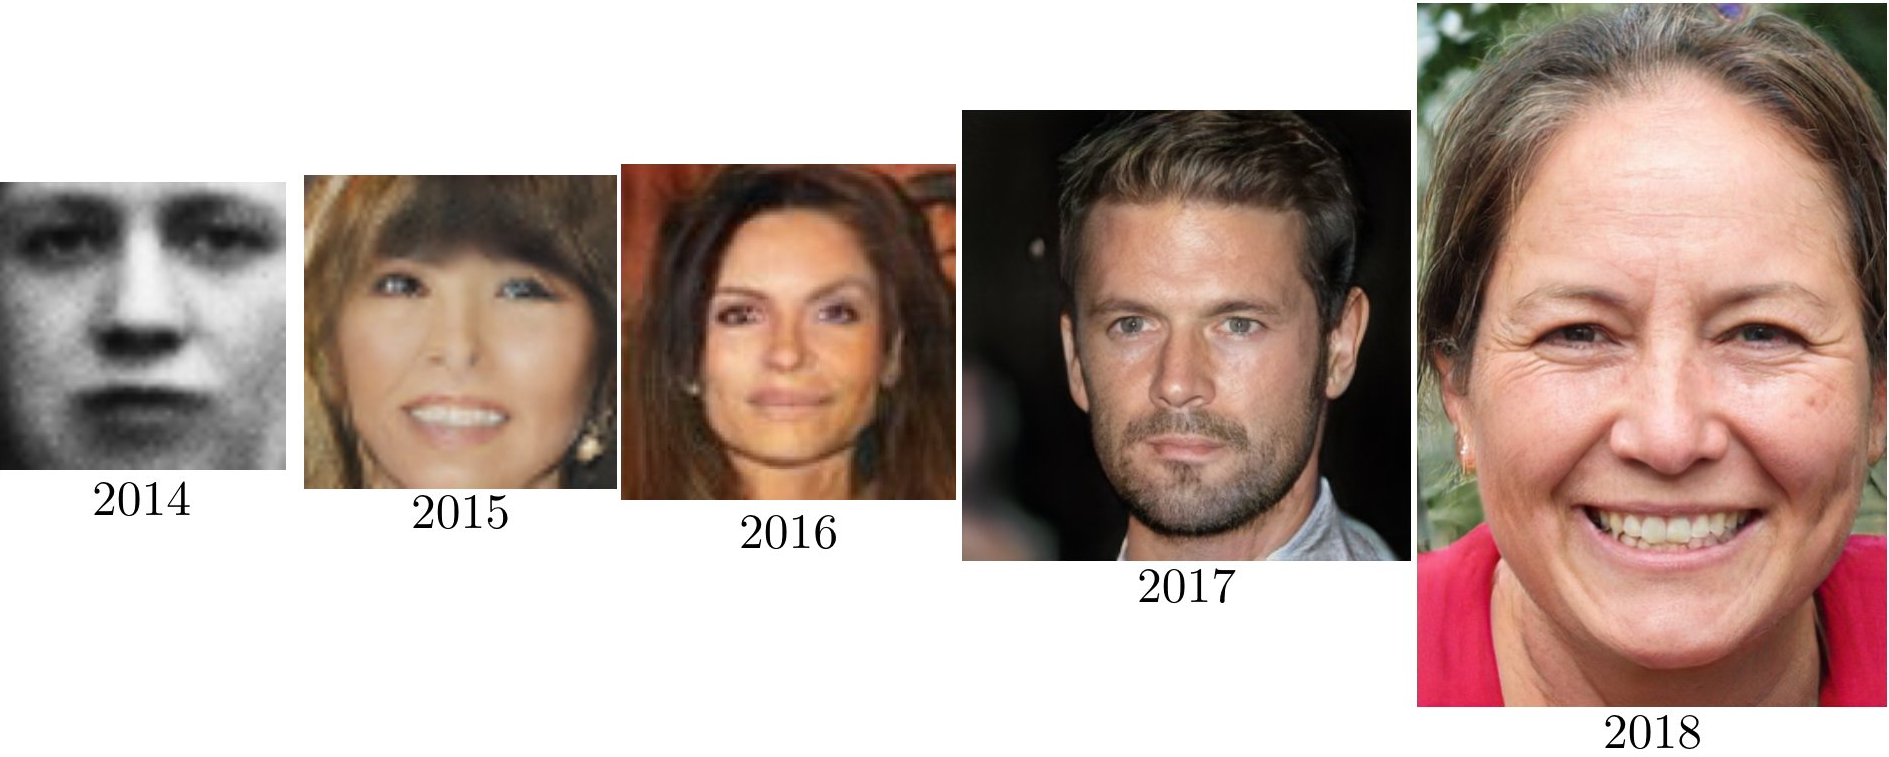
\includegraphics[width=\linewidth]{figs/gan_evolution}
	\end{figure}
	\begin{itemize}
		\item \textbf{Vanilla GAN} \href{https://arxiv.org/abs/1406.2661}{https://arxiv.org/abs/1406.2661}
		\item \textbf{DCGAN} \href{https://arxiv.org/abs/1511.06434}{https://arxiv.org/abs/1511.06434}
		\item \textbf{CoGAN} \href{https://arxiv.org/abs/1606.07536}{https://arxiv.org/abs/1606.07536}
		\item \textbf{ProGAN} \href{https://arxiv.org/abs/1710.10196}{https://arxiv.org/abs/1710.10196} 
		\item \textbf{StyleGAN} \href{https://arxiv.org/abs/1812.04948}{https://arxiv.org/abs/1812.04948}
	\end{itemize}
\end{frame}
%=======
\begin{frame}{Self-Attention GAN}
	\begin{itemize}
		\item Convolutional layers process the information in a local neighborhood.
		\item Using convolutional layers alone is computationally inefficient for modeling long-range dependencies in images.
	\end{itemize}
	\begin{figure}
		\centering
		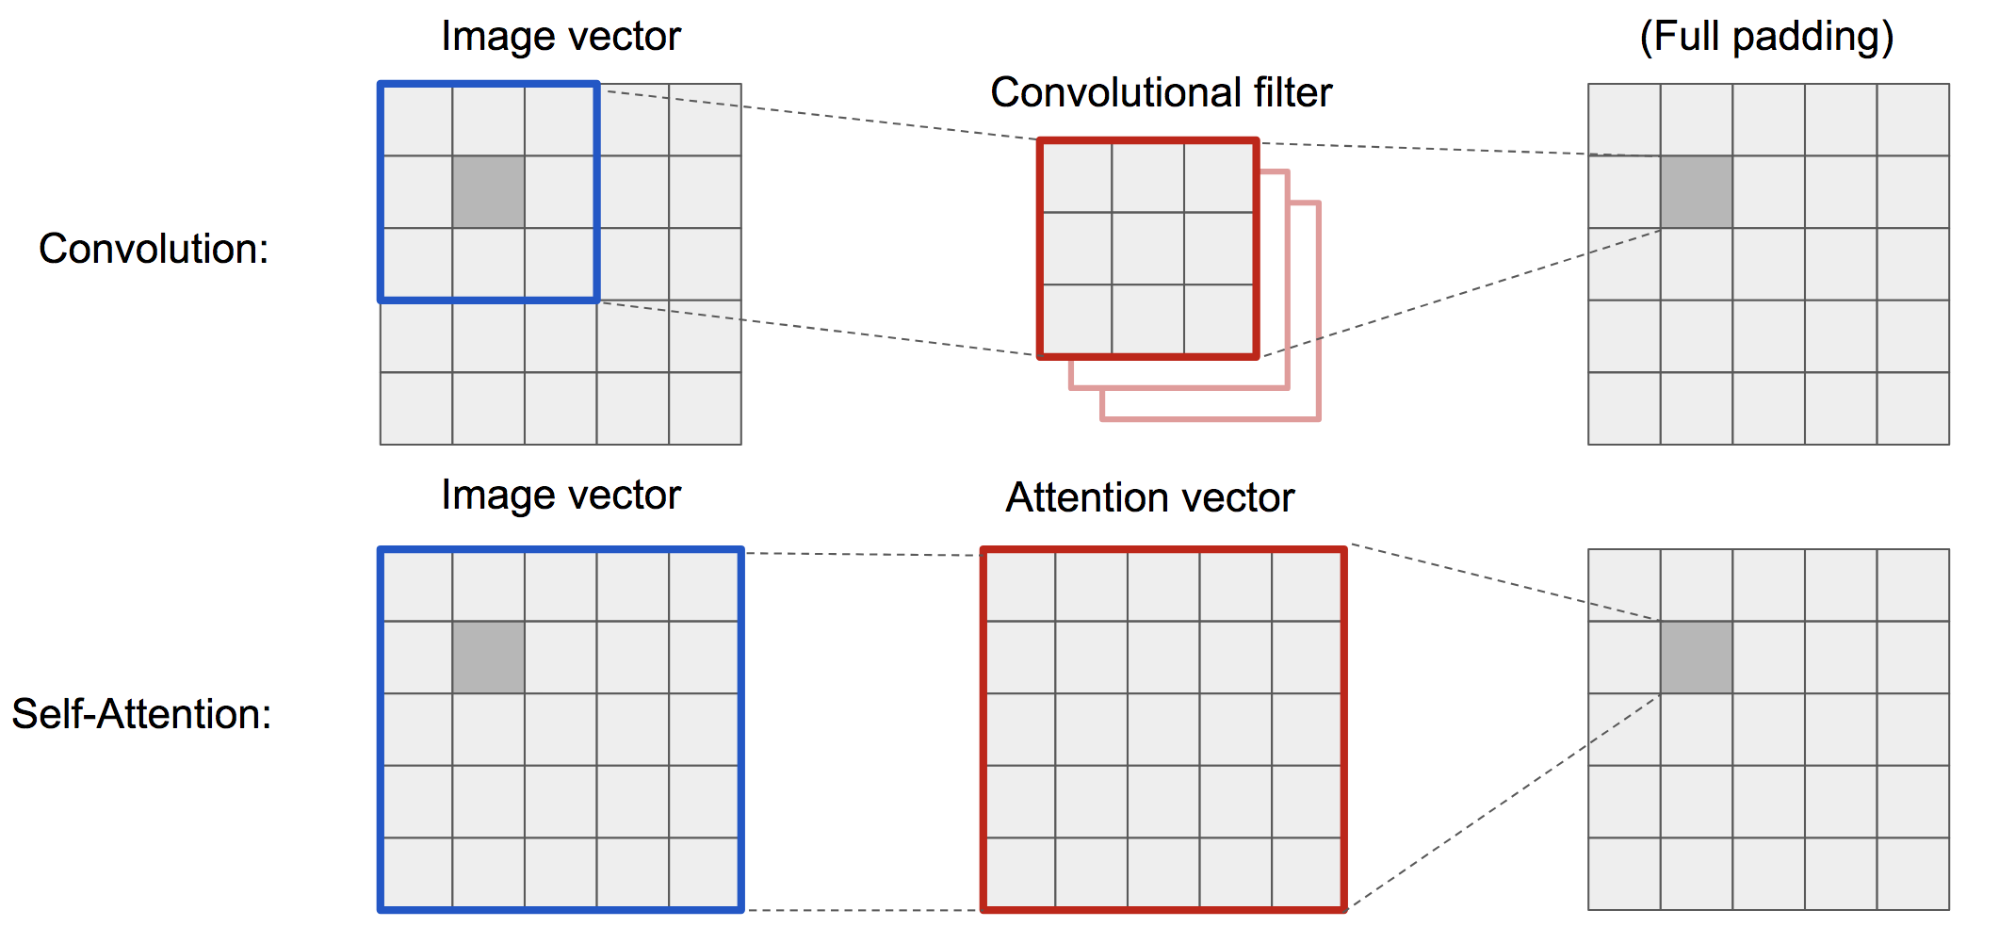
\includegraphics[width=0.9\linewidth]{figs/conv-vs-sa}
	\end{figure}
	\myfootnotewithlink{https://lilianweng.github.io/lil-log/2018/06/24/attention-attention.html}{image credit: https://lilianweng.github.io/lil-log/2018/06/24/attention-attention.html}
\end{frame}
%=======
\begin{frame}{Self-Attention GAN}
	\begin{figure}
		\centering
		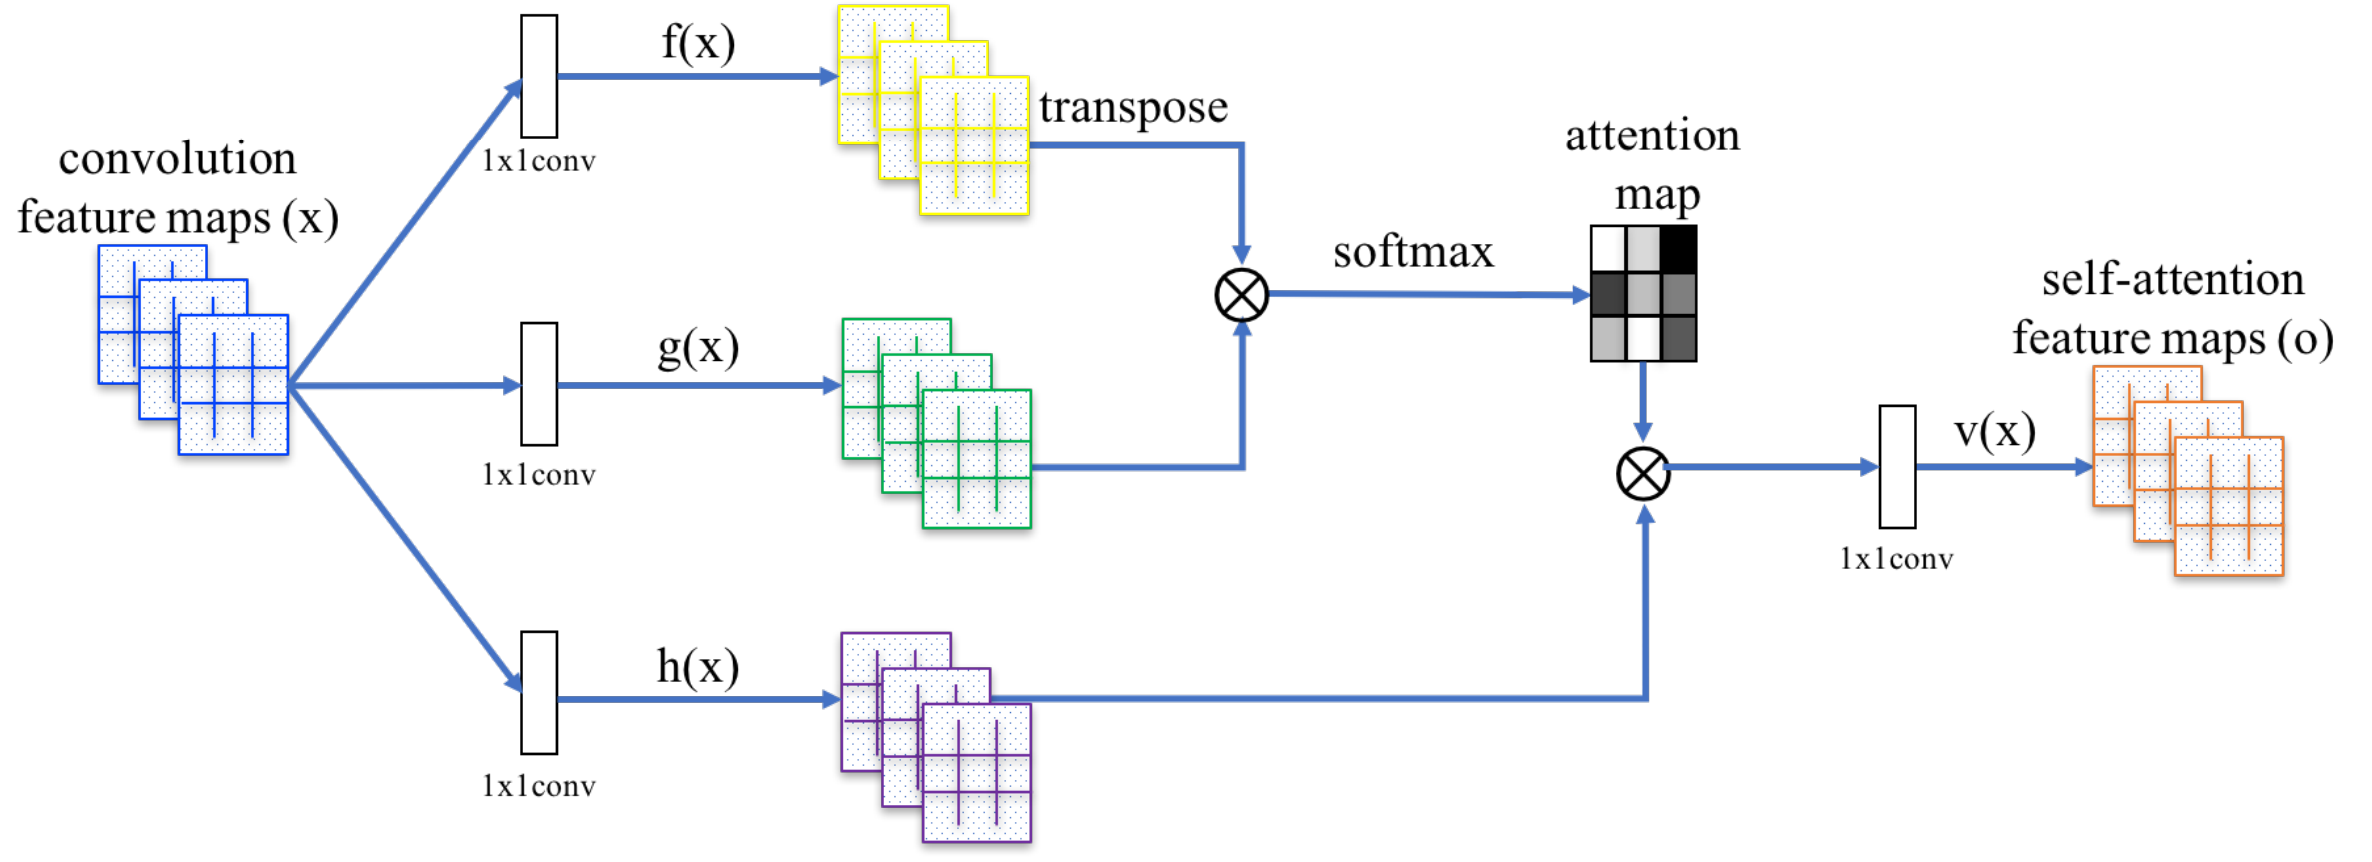
\includegraphics[width=0.9\linewidth]{figs/self-attention}
	\end{figure}
	\vspace{-0.2cm}
	\begin{itemize}
		\item $\bx$ -- feature vector for one feature location.
		\item $N$ -- number of feature locations.
	\end{itemize}
	\vspace{0.5cm}
	\[
		\mathbf{f}(\bx) = \bW_f \bx, \quad \mathbf{g}\bx = \bW_g\bx, \quad \mathbf{h}\bx = \bW_h\bx, \quad \mathbf{v}\bx = \bW_v\bx
	\]
	\[
		s_{ij} = \mathbf{f}(\bx_i)^T \mathbf{g}(\bx_j), \quad a_{ij} = \frac{\exp{s_{ij}}}{\sum_{i=1}^N \exp{s_{ij}}}, \quad \textbf{o}_j = \textbf{v}\left( \sum_{i=1}^N a_{ij} \mathbf{h}(\bx_i) \right)
	\]
	\myfootnotewithlink{https://arxiv.org/abs/1805.08318}{Zhang H. et al. Self-Attention Generative Adversarial Networks, 2018}
\end{frame}
%=======
\begin{frame}{Self-Attention GAN}
	\begin{block}{Technical Details}
		\begin{itemize}
			\item Hinge loss for training.
			\item SpectralNorm in both the generator and the discriminator.
			\item Separate learning rates for the generator and the discriminator.
		\end{itemize}
	\end{block}
	\begin{figure}
		\centering
		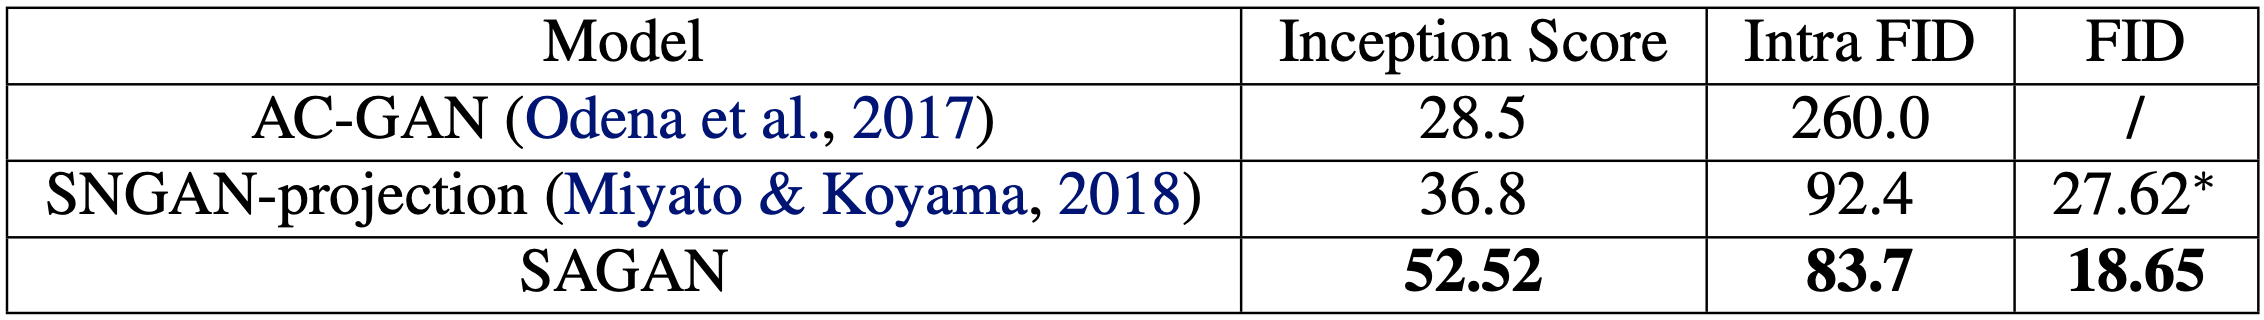
\includegraphics[width=0.85\linewidth]{figs/sa_results2}
	\end{figure}
	\vspace{-0.3cm}
	\begin{block}{Visualization of attention maps}
		\begin{figure}
			\centering
			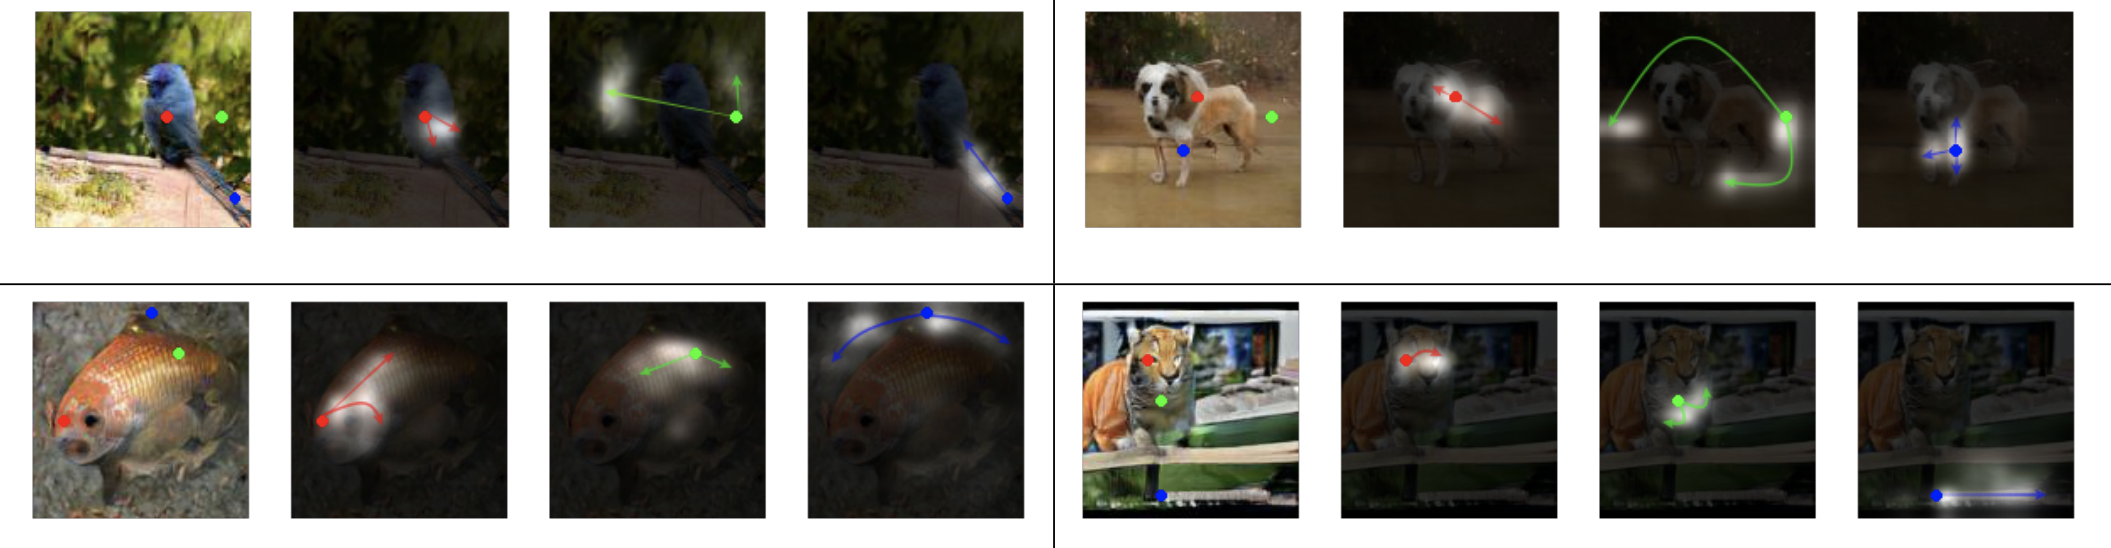
\includegraphics[width=\linewidth]{figs/sa_maps}
		\end{figure}
	\end{block}

	\myfootnotewithlink{https://arxiv.org/abs/1805.08318}{Zhang H. et al. Self-Attention Generative Adversarial Networks, 2018}
\end{frame}
%=======
\begin{frame}{BigGAN}
		\begin{block}{Technical Details}
			\begin{itemize}
				\item Hinge loss.
				\item Self-Attention GAN baseline.
				\item \textbf{Orthogonal regularization}
				\vspace{-0.2cm}
				\[
					\| \bW^T \bW - \bI \|^2 \quad \Rightarrow \quad \| \bW^T \bW - \text{diag}(\bW^T \bW) \|^2
				\]
				\vspace{-0.8cm}
				\item \textbf{Truncation trick.} Components of $\bz \sim \cN(0, \bI)$ which fall outside a predefined range are resampled.
			\end{itemize}
		\end{block}
	\begin{figure}
		\centering
		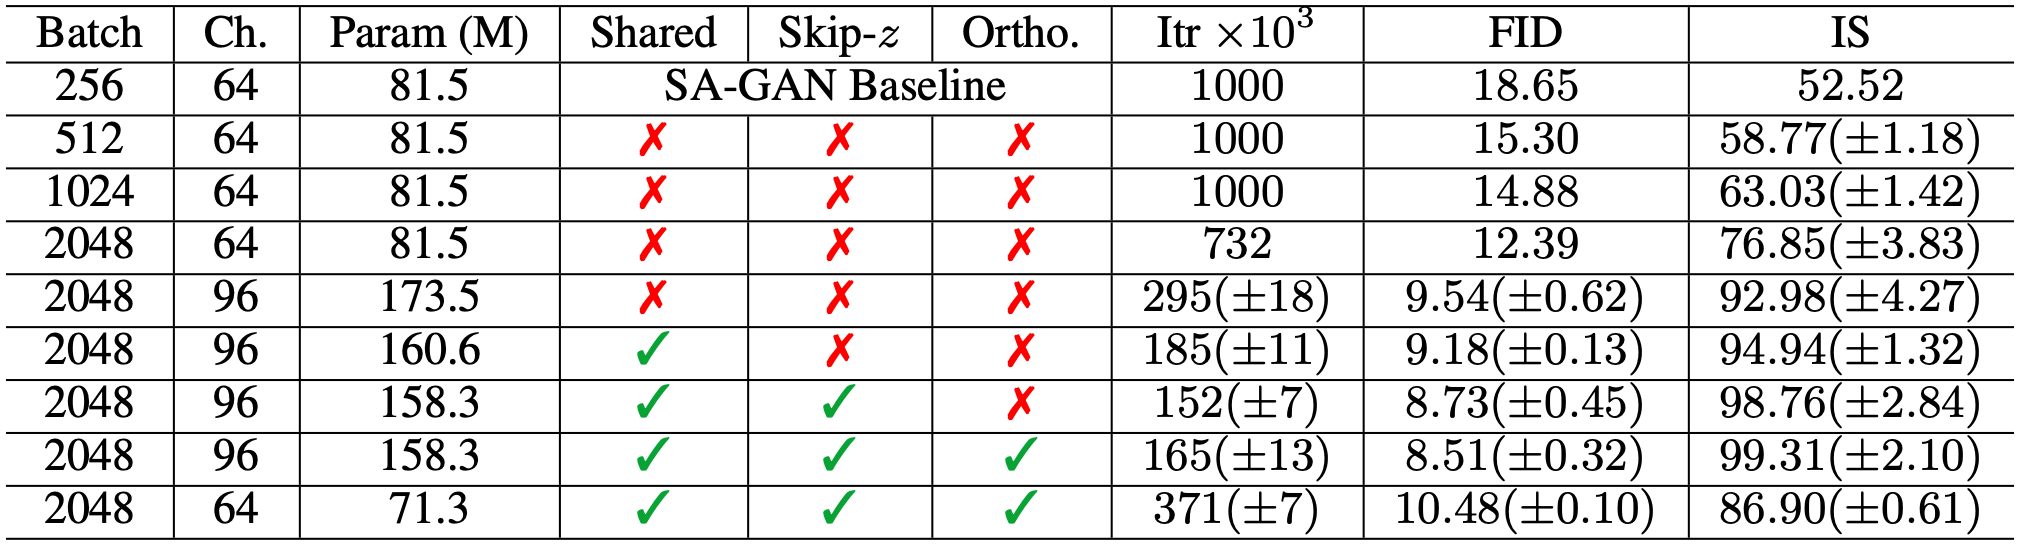
\includegraphics[width=\linewidth]{figs/biggan_results}
	\end{figure}
	
	\myfootnotewithlink{https://arxiv.org/abs/1809.11096}{Brock A., Donahue J., Simonyan K. Large Scale GAN Training for High Fidelity Natural Image Synthesis, 2018}
\end{frame}
%=======
\begin{frame}{BigGAN}
	\begin{block}{Samples (512x512)}
		\begin{figure}
			\centering
			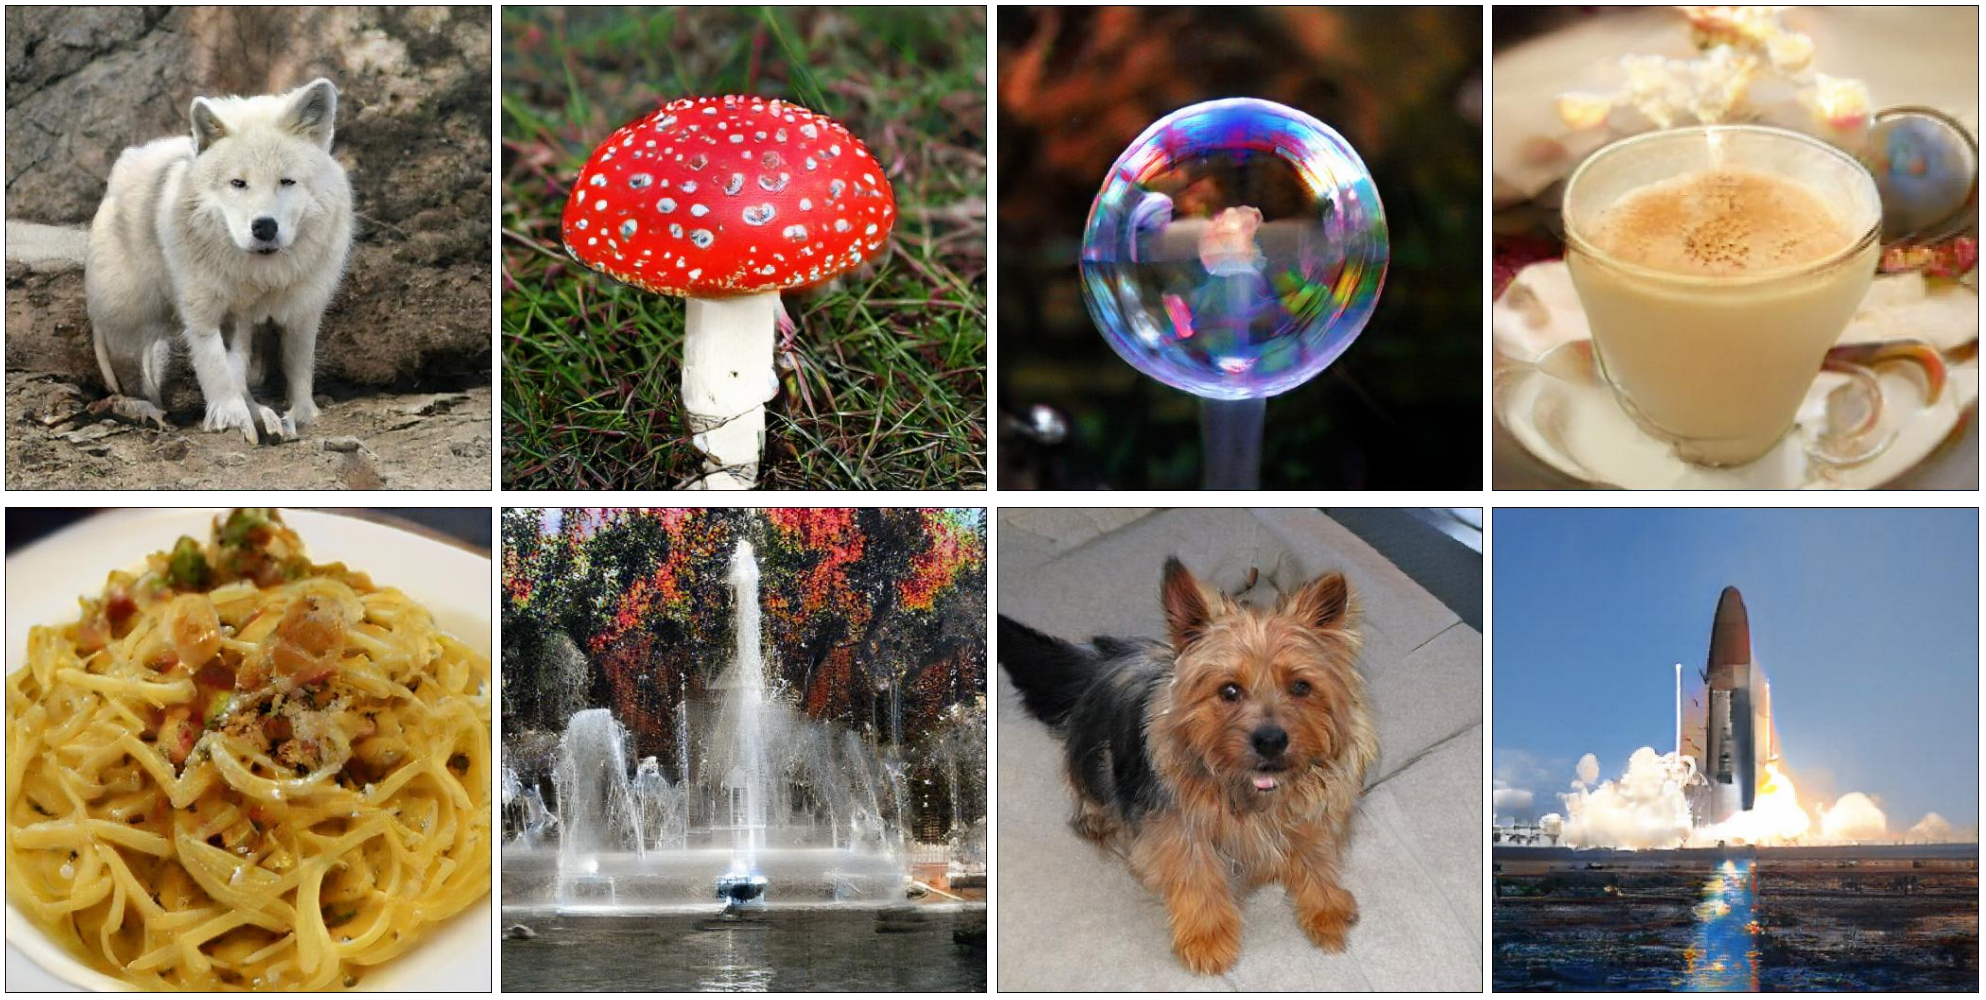
\includegraphics[width=\linewidth]{figs/biggan_samples}
		\end{figure}
	\end{block}
	\vspace{-0.4cm}
	\begin{block}{Interpolations}
		\begin{figure}
			\centering
			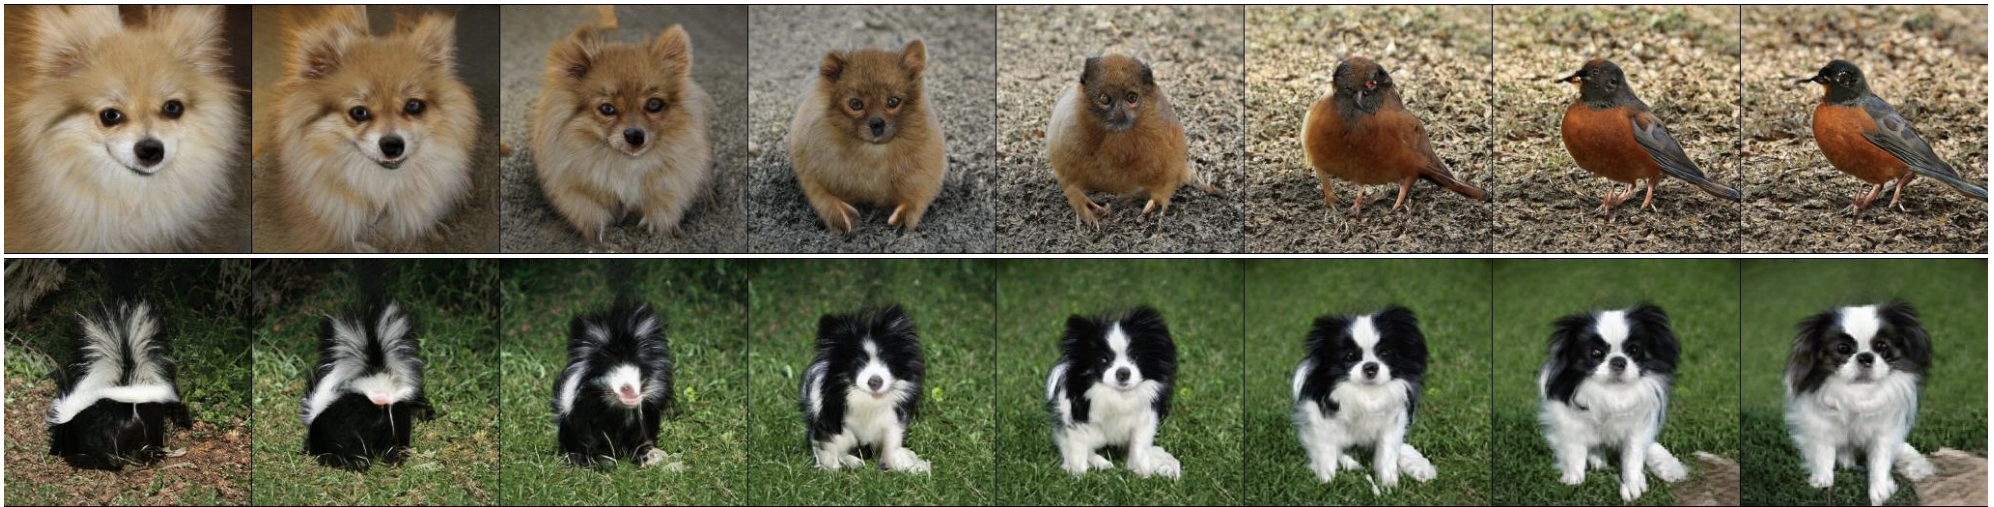
\includegraphics[width=\linewidth]{figs/biggan_interpolations}
		\end{figure}
	\end{block}
	\myfootnotewithlink{https://arxiv.org/abs/1809.11096}{Brock A., Donahue J., Simonyan K. Large Scale GAN Training for High Fidelity Natural Image Synthesis, 2018}
\end{frame}
%=======
\begin{frame}{Progressive Growing GAN}
	\begin{block}{Problems with HR image generation}
		\begin{itemize}
			\item Disjoint manifolds $\Rightarrow$ gradient problem.
			\item Small minibatch $\Rightarrow$ training instability.
		\end{itemize}
	\end{block}
	\vspace{-0.2cm}
	\begin{block}{Samples (1024x1024)}
		\vspace{-0.2cm}
		\begin{figure}
			\includegraphics[width=0.9\linewidth]{figs/pggan_samples}
		\end{figure}
	\end{block}
	\myfootnotewithlink{https://arxiv.org/abs/1710.10196}{Karras T. et al. Progressive Growing of GANs for Improved Quality, Stability, and Variation, 2017}
\end{frame}
\begin{frame}{Progressive Growing GAN}
	Grow both the generator and discriminator progressively, new layers will introduce higher-resolution details as the training progresses. 
	\begin{itemize}
		\item Train GAN which generate 4x4 images (2 convs for G and D).
		\item Add upsampling layers to G, downsampling layers to D.
		\item Train GAN which generate 8x8 images.
		\item etc.
	\end{itemize}
	\vspace{-0.2cm}
	\begin{figure}
		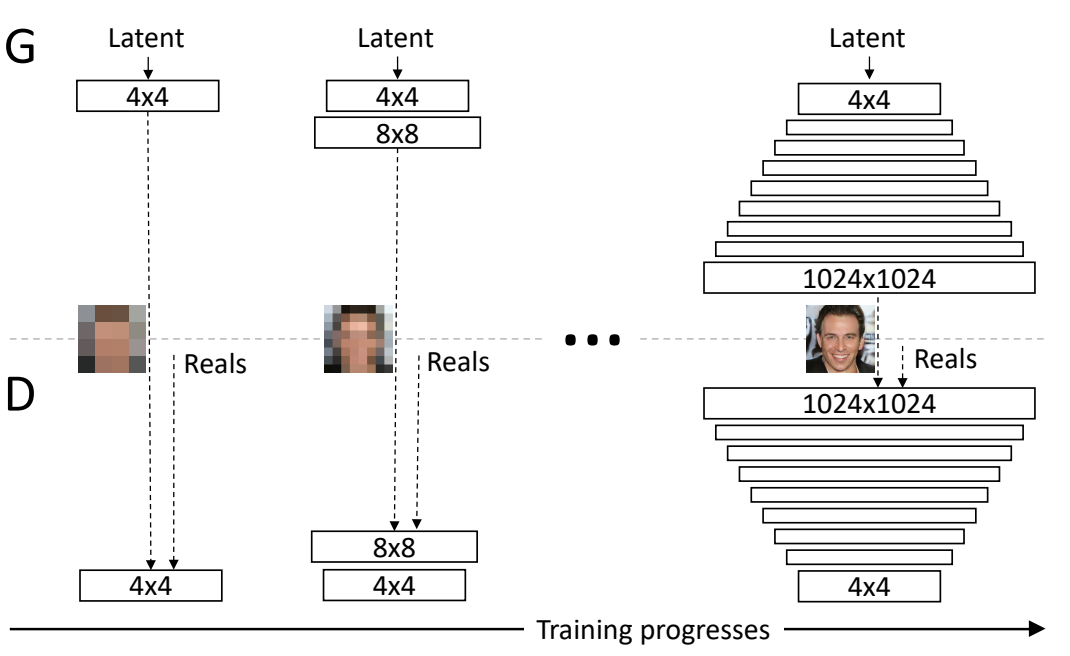
\includegraphics[width=0.75\linewidth]{figs/pggan_arch}
	\end{figure}

	\myfootnotewithlink{https://arxiv.org/abs/1710.10196}{Karras T. et al. Progressive Growing of GANs for Improved Quality, Stability, and Variation, 2017}
\end{frame}
%=======
\begin{frame}{StyleGAN}
	\begin{itemize}
		\item Generating of HR images is hard.
		\item Progressive growing greatly simplifies the task.
		\item The ability to control specific features of the generated image is very limited.
	\end{itemize}
	\begin{block}{Face image features}
		\begin{itemize}
			\item Coarse (pose, general hair style, face shape). Resolution $4^2 - 8^2$.
			\item Middle (finer facial features, hair style, eyes open/closed). Resolution $16^2 - 32^2$.
			\item Fine (color scheme (eye, hair and skin) and micro features). Resolution $64^2 - 1024^2$.
		\end{itemize}
	\end{block}
	\myfootnotewithlink{https://arxiv.org/abs/1812.04948}{Karras T., Laine S., Aila T. A Style-Based Generator Architecture for Generative Adversarial Networks, 2018}
\end{frame}
%=======
\begin{frame}{StyleGAN}
	\begin{block}{Mapping Network}
		\begin{itemize}
			\item Generator input is likely to be \textbf{disentangled}.  Each component of input vector $\bz$ should be responsible for one generative factor.
			\item Mapping network $f: \cZ \rightarrow \cW$ is used to reduce correlations between components of~$\bz$.
		\end{itemize}
		\begin{minipage}[t]{0.6\columnwidth}
			\begin{figure}
				\centering
				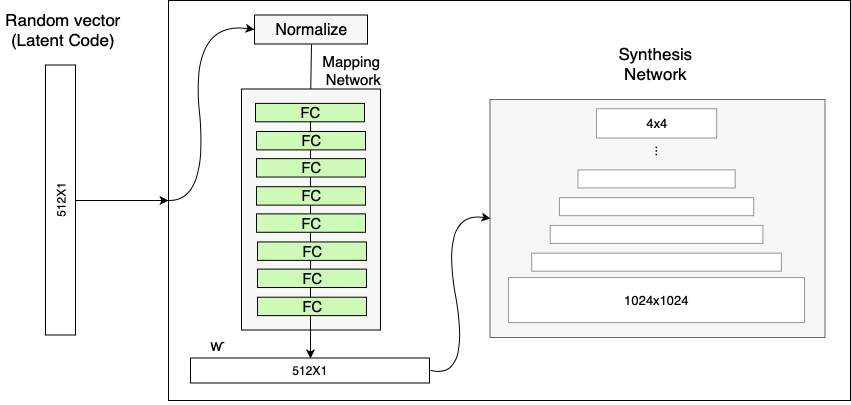
\includegraphics[width=0.98\linewidth]{figs/stylegan_mapping}
			\end{figure}
		\end{minipage}%
		\begin{minipage}[t]{0.38\columnwidth}
			\begin{figure}
				\centering
				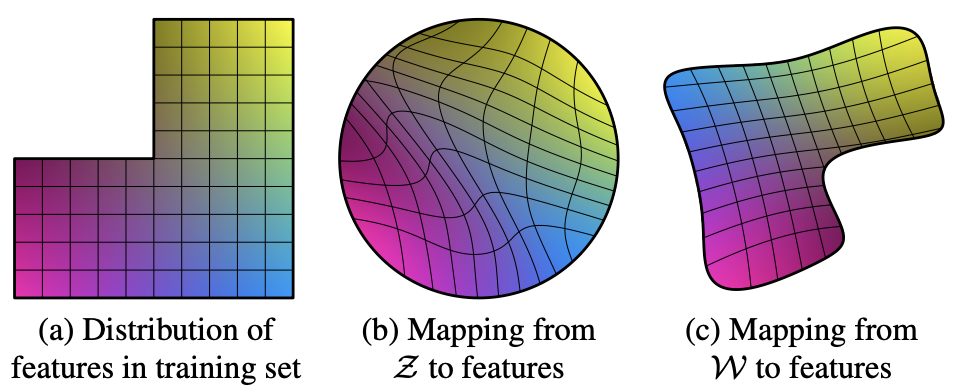
\includegraphics[width=1.0\linewidth]{figs/stylegan_curved}
			\end{figure}
		\end{minipage}
	\vspace{0.3cm}
	\end{block}

	\myfootnotewithlink{https://arxiv.org/abs/1812.04948}{Karras T., Laine S., Aila T. A Style-Based Generator Architecture for Generative Adversarial Networks, 2018}
\end{frame}

\begin{frame}{StyleGAN}
	\begin{block}{Truncation trick}
		\vspace{-0.2cm}
		\[
			\bw' = \hat{\bw} + \psi \cdot (\bw - \hat{\bw}), \quad \hat{\bw} = \bbE_{\bz} p(f(\bz))
		\]
		\vspace{-0.2cm}
		\begin{itemize}
			\item Constant $\psi$ is a tradeoff between diversity and fidelity. 
			\item $\psi=0.7$ is used for most of the results.
			\item Truncation is done only at the low-resolution layers.
		\end{itemize}
		\begin{figure}
			\centering
			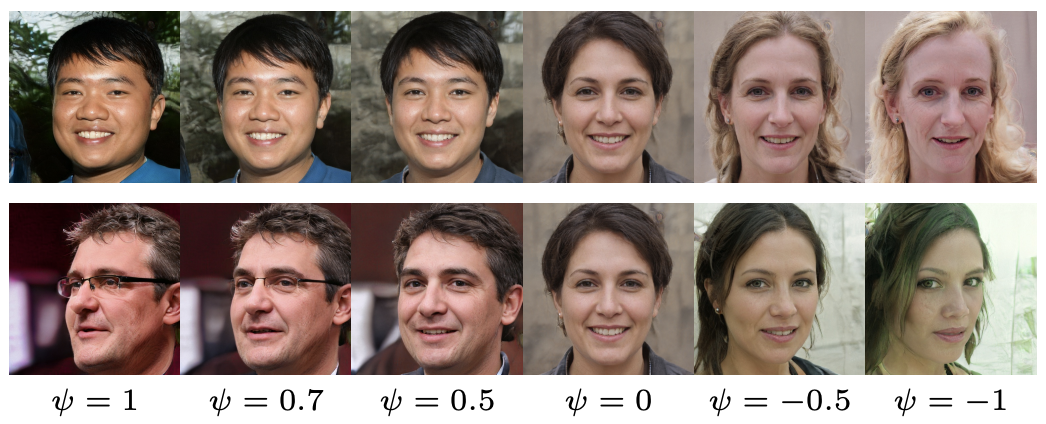
\includegraphics[width=0.8\linewidth]{figs/stylegan_truncation}
		\end{figure}
	\end{block}

	\myfootnotewithlink{https://arxiv.org/abs/1812.04948}{Karras T., Laine S., Aila T. A Style-Based Generator Architecture for Generative Adversarial Networks, 2018}
\end{frame}
%=======
\begin{frame}{StyleGAN}
	\begin{block}{Results}
		\vspace{-0.2cm}
		\begin{figure}
			\centering
			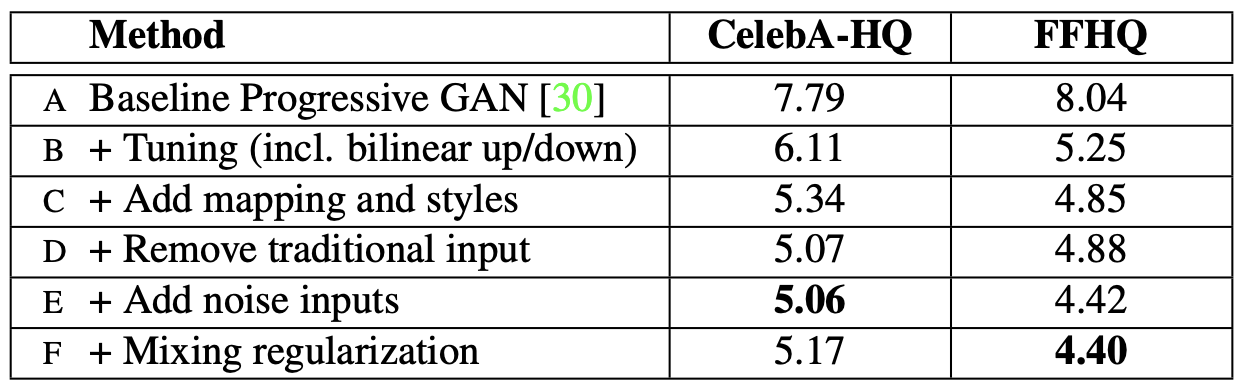
\includegraphics[width=0.6\linewidth]{figs/stylegan_results}
		\end{figure}
	\vspace{-0.3cm}
	\end{block}
	\begin{block}{Samples (1024x1024)}
		\begin{figure}
			\centering
			\includegraphics[width=0.8\linewidth]{figs/stylegan_samples}
		\end{figure}
	\vspace{-0.1cm}
	\end{block}

	\myfootnotewithlink{https://arxiv.org/abs/1812.04948}{Karras T., Laine S., Aila T. A Style-Based Generator Architecture for Generative Adversarial Networks, 2018}
\end{frame}
%=======
\begin{frame}{VAE recap}
	\vspace{-0.3cm}
	\begin{figure}[h]
		\centering
		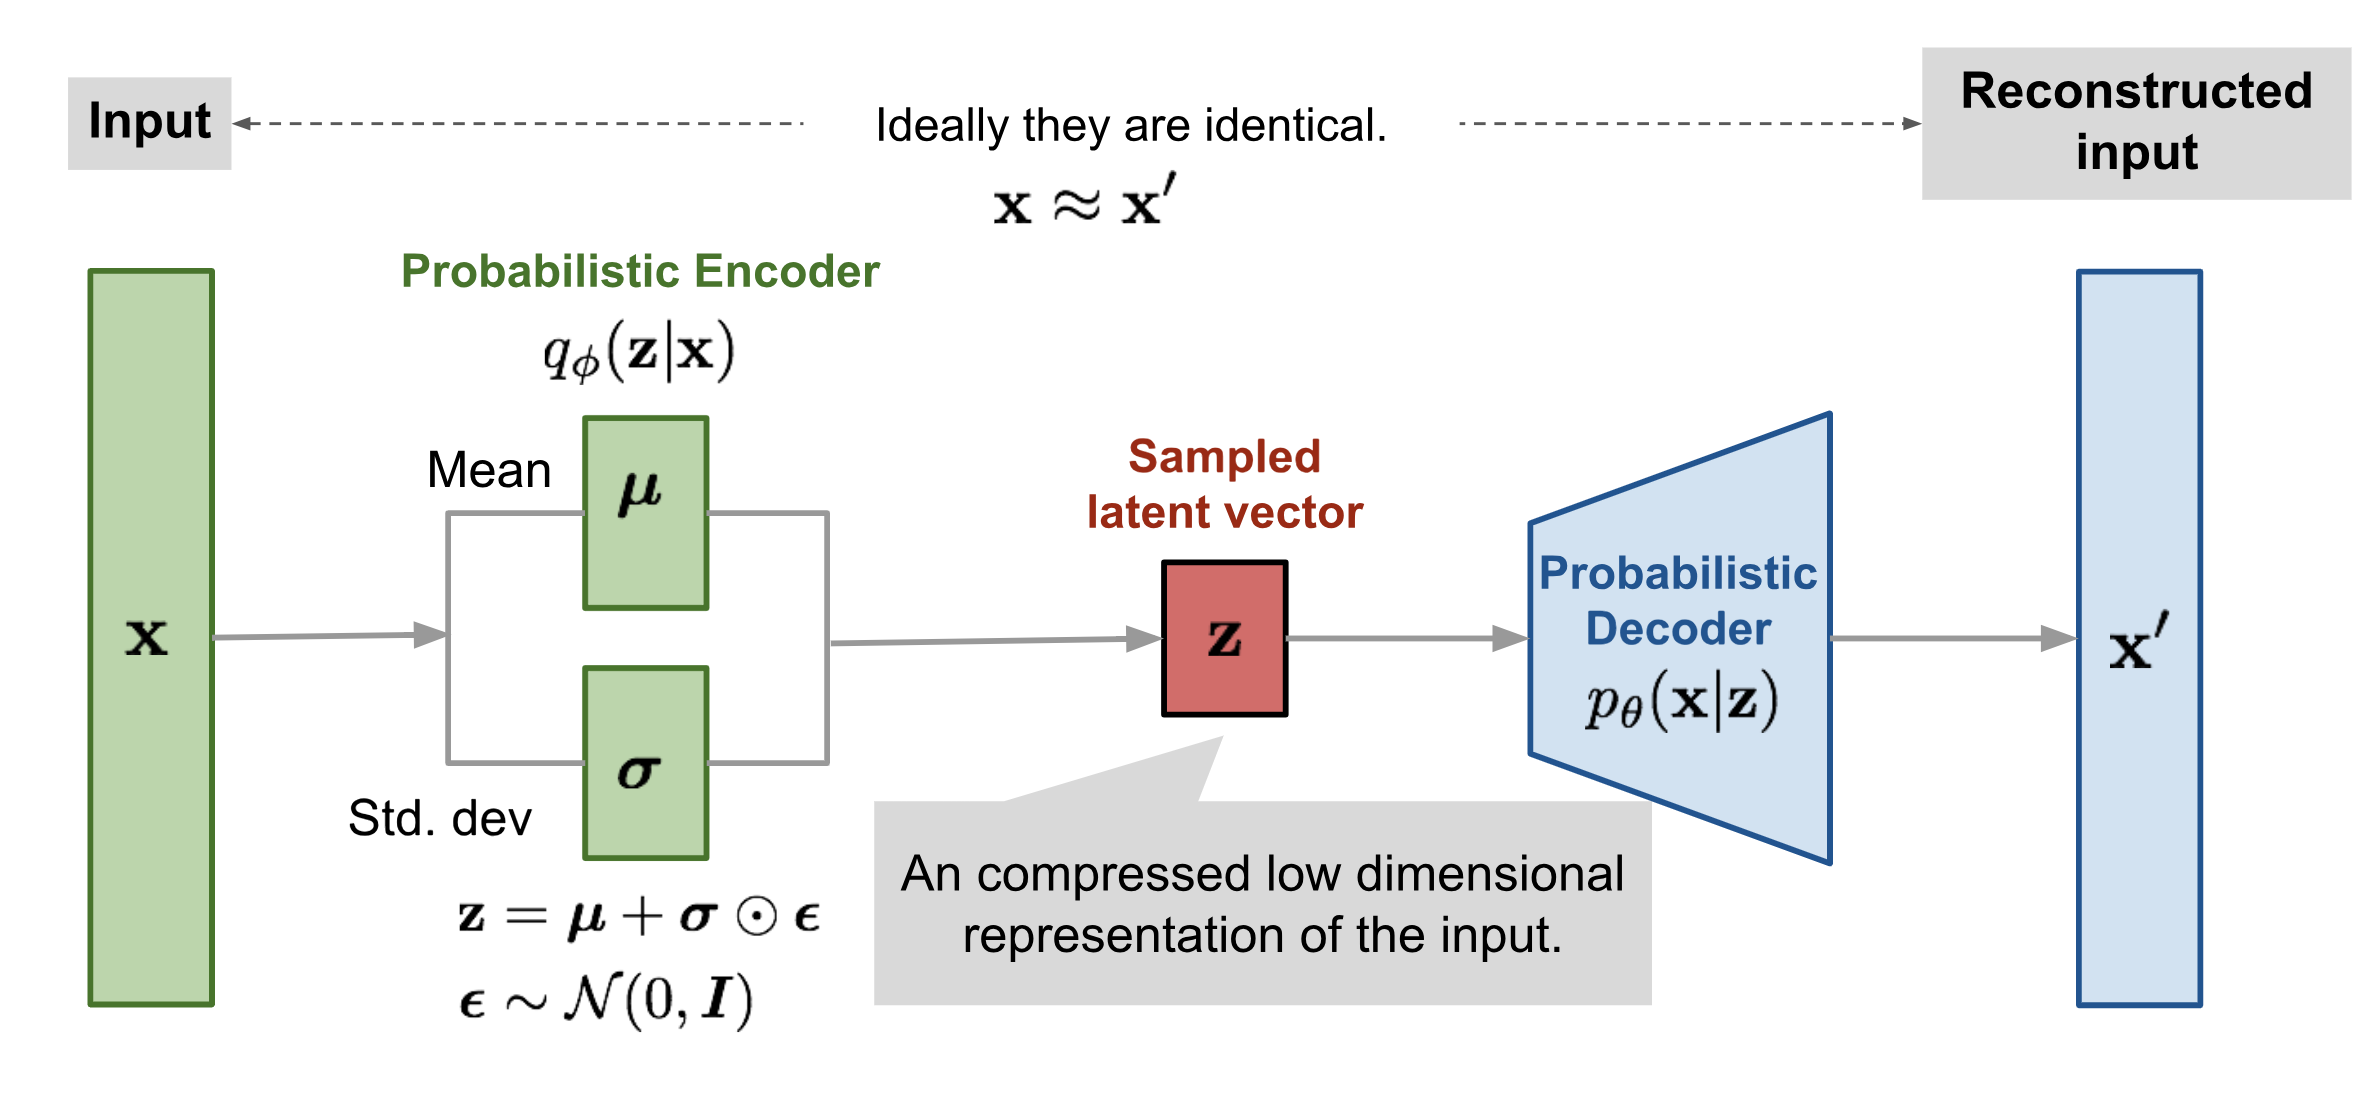
\includegraphics[width=\linewidth]{figs/vae-gaussian.png}
	\end{figure}
	\vspace{-0.5cm}
	\begin{itemize}
		\item Encoder $q(\bz | \bx, \bphi) = \cN(\bz | \bmu_{\bphi}(\bx), \bsigma_{\bphi}(\bx))$.
		\item Variational posterior $q(\bz | \bx, \bphi)$ originally approximates the true posterior $p(\bz | \bx, \btheta)$.
		\item Which methods are you already familiar with to make the posterior is more flexible?
	\end{itemize}
	\myfootnotewithlink{https://lilianweng.github.io/lil-log/2018/08/12/from-autoencoder-to-beta-vae.html}{image credit: https://lilianweng.github.io/lil-log/2018/08/12/from-autoencoder-to-beta-vae.html}
\end{frame}
%=======
\begin{frame}{Adversarial Variational Bayes}
	\begin{block}{ELBO objective}
		\vspace{-0.5cm}
		\[
			 \mathcal{L} (\bphi, \btheta)  = \mathbb{E}_{q(\bz | \bx, \bphi)} \left[\log p(\bx | \bz, \btheta) + \log p(\bz) - \log q(\bz| \bx, \bphi) \right] \rightarrow \max_{\bphi, \btheta}.
		\]	
		\vspace{-0.5cm}
	\end{block}
	What is the problem to make the variational posterior model an implicit model?
	\begin{itemize}
	\item The first term is reconstruction loss that needs only samples from $q(\bz | \bx, \bphi)$ to evaluate.
	\item Reparametrization trick allows to get gradients of reconstruction loss
		\vspace{-0.4cm}
		\begin{multline*}
			\nabla_{\bphi}\int q(\bz|\bx, \bphi) f(\bz) d\bz = \nabla_{\bphi}\int r(\bepsilon)  f(\bz) d\bepsilon \\ = \int r(\bepsilon) \nabla_{\bphi} f(g(\bx, \bepsilon, \bphi)) d\bepsilon \approx \nabla_{\bphi} f(g(\bx, \bepsilon^*, \bphi)),
		\end{multline*}
		\vspace{-0.6cm} \\
		where $\bepsilon^* \sim r(\bepsilon), \quad \bz = g(\bx, \bepsilon, \bphi), \quad \bz \sim q(\bz | \bx, \bphi)$.
	\end{itemize}
	\myfootnotewithlink{https://arxiv.org/abs/1701.04722}{Mescheder L., Nowozin S., Geiger A. Adversarial variational bayes: Unifying variational autoencoders and generative adversarial networks, 2017}
\end{frame}
%=======
\begin{frame}{Adversarial Variational Bayes}
	\begin{block}{ELBO objective}
		\vspace{-0.5cm}
		\[
			 \mathcal{L} (\bphi, \btheta)  = \mathbb{E}_{q(\bz | \bx, \bphi)} \left[\log p(\bx | \bz, \btheta) + \log p(\bz) - \log q(\bz| \bx, \bphi) \right] \rightarrow \max_{\bphi, \btheta}.
		\]	
		\vspace{-0.5cm}
	\end{block}
	What is the problem to make the variational posterior model an implicit model?
	\begin{itemize}
	\item The third term requires the ability to calculate the value of $q(\bz | \bx, \bphi)$.
	\item We could join second and third terms:
		\vspace{-0.2cm}
		\[
			\mathbb{E}_{q(\bz | \bx, \bphi)} \log \frac{p(\bz)}{q(\bz| \bx, \bphi)} = \mathbb{E}_{q(\bz | \bx, \bphi)} \log \frac{p(\bz) \pi(\bx)}{q(\bz| \bx, \bphi) \pi (\bx)}.
		\]
		\vspace{-0.5cm}
	\item We have to estimate density ratio 
		\vspace{-0.2cm}
		\[
			r(\bx, \bz) = \frac{q_1(\bx, \bz)}{q_2(\bx, \bz)} = \frac{p(\bz) \pi(\bx)}{q(\bz| \bx, \bphi) \pi (\bx)}.
		\] 
	\end{itemize}
	\myfootnotewithlink{https://arxiv.org/abs/1701.04722}{Mescheder L., Nowozin S., Geiger A. Adversarial variational bayes: Unifying variational autoencoders and generative adversarial networks, 2017}
\end{frame}
%=======
\begin{frame}{Density ratio trick}
	Consider two distributions $q_1(\bx)$, $q_2(\bx)$ and probabilistic model
	\[
		p(\bx | y) = \begin{cases}
			q_1(\bx), \text{ if } y = 1, \\
			q_2(\bx), \text{ if } y = 0,
		\end{cases}
		\quad 
		y \sim \text{Bern}(0.5).
	\]
	\vspace{-0.3cm}
	\begin{block}{Density ratio}
		\vspace{-0.7cm}
		{\small
		\begin{multline*}
			\frac{q_1(\bx)}{q_2(\bx)} = \frac{p(\bx | y = 1)}{p(\bx | y = 0)} = \frac{p(y = 1 | \bx) p(\bx)}{p(y=1)} \bigg/ \frac{p(y = 0 | \bx) p(\bx)}{p(y=0)} = \\
			= \frac{p(y = 1 | \bx)}{p(y = 0 | \bx)} = \frac{p(y = 1 | \bx)}{1 - p(y = 1 | \bx)} = \frac{D(\bx)}{1 - D(\bx)}
		\end{multline*}
		}
		Here $D(\bx)$ is a discriminator model the output of which is a probability that $\bx$ is a sample
		from $q_1(\bx)$ rather than from $q_2(\bx)$.
	\end{block}
	\begin{block}{Adversarial Variational Bayes}
		\vspace{-0.6cm}
		\[
			\max_D \left[ \bbE_{\pi(\bx)} \bbE_{q(\bz | \bx, \bphi)} \log D(\bx, \bz) + \bbE_{\pi(\bx)} \bbE_{p(\bz)} \log (1 - D(\bx, \bz)) \right]
		\]
	\end{block}
	\myfootnotewithlink{https://arxiv.org/abs/1701.04722}{Mescheder L., Nowozin S., Geiger A. Adversarial variational bayes: Unifying variational autoencoders and generative adversarial networks, 2017}
\end{frame}
%=======
\begin{frame}{Adversarial Variational Bayes}
	\begin{block}{ELBO objective}
		\vspace{-0.5cm}
		\[
			 \mathcal{L} (\bphi, \btheta)  = \mathbb{E}_{q(\bz | \bx, \bphi)} \left[\log p(\bx | \bz, \btheta) + \log \frac{p(\bz)}{q(\bz| \bx, \bphi)} \right] \rightarrow \max_{\bphi, \btheta}.
		\]	
		\vspace{-0.5cm}
	\end{block}
	\begin{figure}
		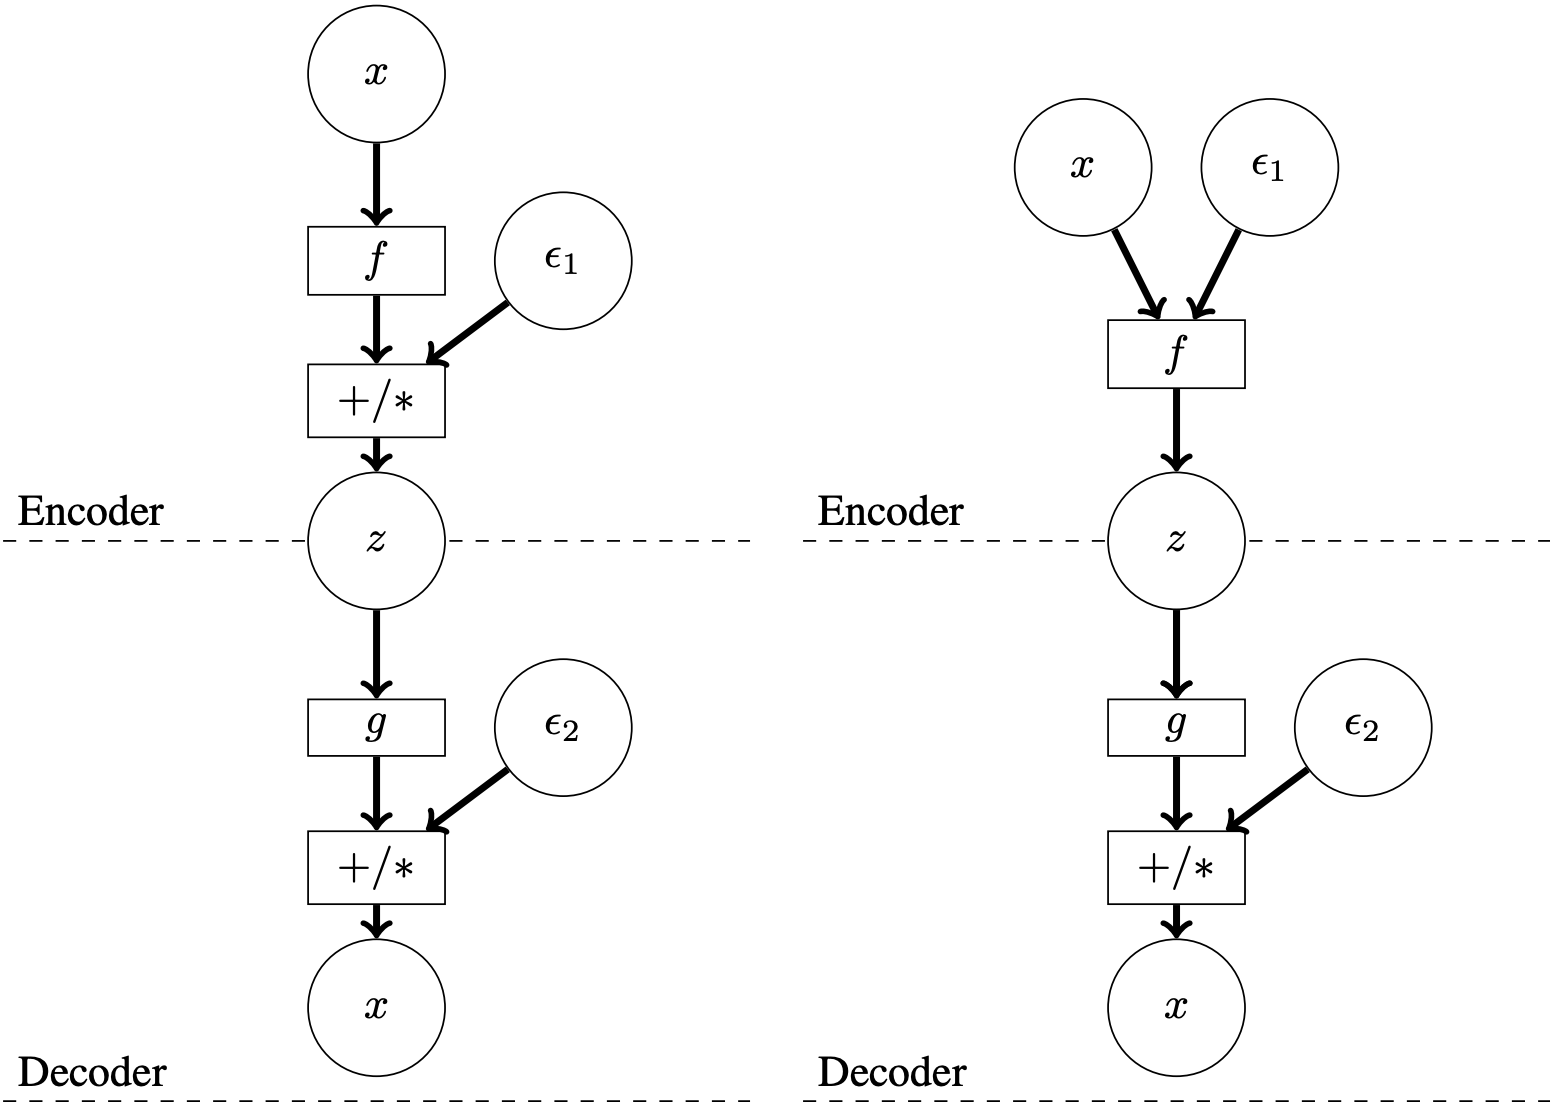
\includegraphics[width=0.7\linewidth]{figs/avb_scheme}
	\end{figure}
	\myfootnotewithlink{https://arxiv.org/abs/1701.04722}{Mescheder L., Nowozin S., Geiger A. Adversarial variational bayes: Unifying variational autoencoders and generative adversarial networks, 2017}
\end{frame}
%=======
\begin{frame}{Summary}
\end{frame}
%=======
\end{document} 